\documentclass[12pt,pdftex]{article}
\usepackage{amsmath}
\usepackage{graphicx}
\usepackage{natbib}
\citestyle{elsart-harv}
\usepackage{rotating}
\usepackage{lineno} 
\usepackage{longtable}
\usepackage{amsmath}
\usepackage{amssymb}
\usepackage{subcaption}

% Text layout
\topmargin 0.0cm
\oddsidemargin 0.5cm
\evensidemargin 0.5cm
\textwidth 16cm 
\textheight 21cm

% Leave date blank
\date{}

\title{Supplementary information\\ Conditions for successful range shifts}
                                                                  
\author{Jonatan \r{A}revall$^{1}$,  Regan Early $^{2}$, Uno Wennergern$^{1}$ \& Anna Ekl\"{o}f$^{1*}$,\\
  $^1$\small Department of Physics, Chemistry and Biology, Division of Theoretical Biology\\
  $^2$\small Centre for Ecology and Conservation, University of Exeter Penryn Campus, Cornwall, UK\\
  $^*$ \small Corresponding author: anna.eklof@liu.se\\
}
\begin{document}
\linenumbers
\maketitle
\baselineskip 18pt

\section*{Empirical data for dispersal}
As a basis for the model we use dispersal data for eight mammals found in Europe \citep{Whitmee2013}. The species’ natal dispersal distances was used to calculate the dispersal kernels for a landscape of size 50x50 km

\section*{Calculating dispersal kernels for empirical data}
As a basis for the model we use dispersal data for eight mammals found in Europe \citep{Whitmee2013}. The dispersal kernel shows the probability distribution of the distance traveled by any individual. The species’ natal dispersal distance was used to calculate the dispersal kernels for the eight mammal species for a landscape of size 50x50 km. The dispersal data used  is the distance where the 99\% percentile of dispersed individuals is found. We start the calculations by normalizing the data, e.g., if 99\% dispersal for a species is 17.353 km and the landscape size 50x50 km then the normalized values for dispersal is 17.353/50 = 0.34706 in a 1x1 landscape. Equation for the dispersal kernel is 

\begin{equation}
p(distance) = e^{-(distance/a)}
\end{equation}

assuming $b$ is 1. 
Since the dispersal distance $d$ here is the distance where 99\% of dispersers are found within, the integral up until this distance will be equal to the infinite integral multiplied by 0.99. This expression gives the following equation:

\begin{equation}
F(d) - F(0) =  (F(long) - F(0)) \times 0.99
\end{equation}

\begin{equation}
-a*e^{-(d/a)}+a = (-a*e^{-(x/a)}+a) * 0.99           
\end{equation}
 when x is large. Solving this expression numerically yields an $a$-value for the species and from that the dispersal kernel can be derived using Eq X.


\section*{Classes of heterogeneous landscapes}
We divided the heterogeneous landscapes in three classes based on the fraction of habitat positioned in middle third of the landscape: A - 0--23\%, B) 23--43\%  and C) 43--100\% (for visualization see Fig. S1). 

\begin{figure}[h]
\begin{subfigure}{.32\textwidth}
  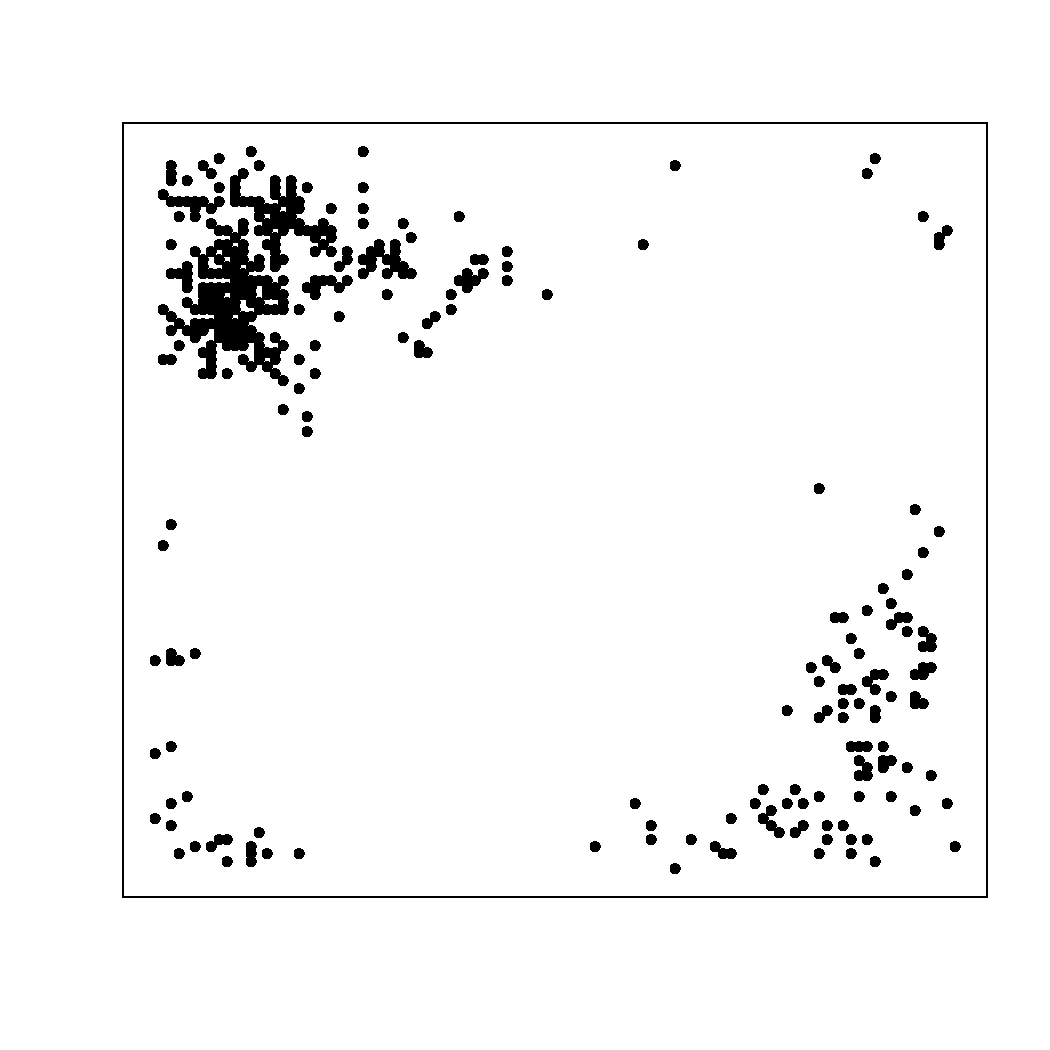
\includegraphics[width=1.9in]{../Figures/example_6A.pdf}
  \caption{}
\end{subfigure}
\begin{subfigure}{.32\textwidth}
  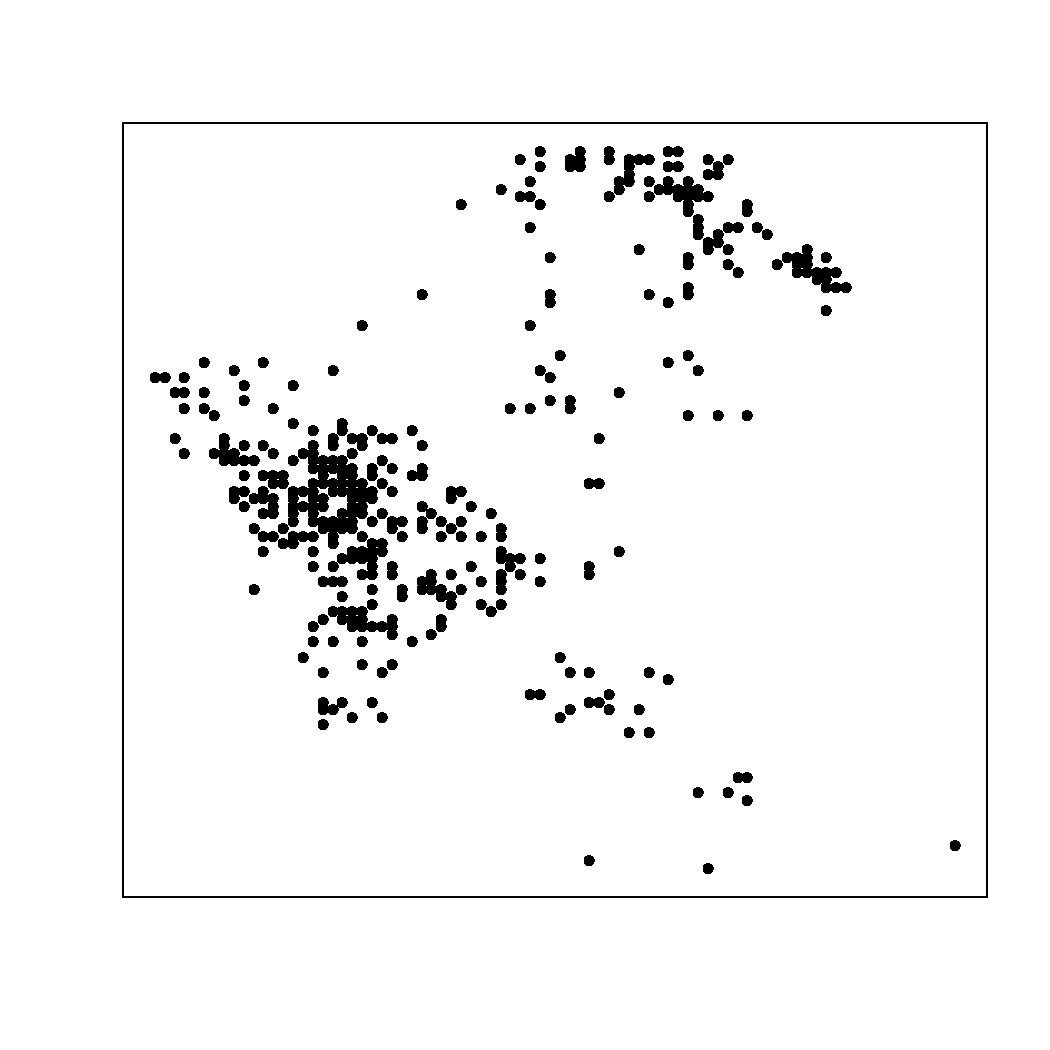
\includegraphics[width=1.9in]{../Figures/example_6B.pdf}
  \caption{}
\end{subfigure}
\begin{subfigure}{.32\textwidth}
  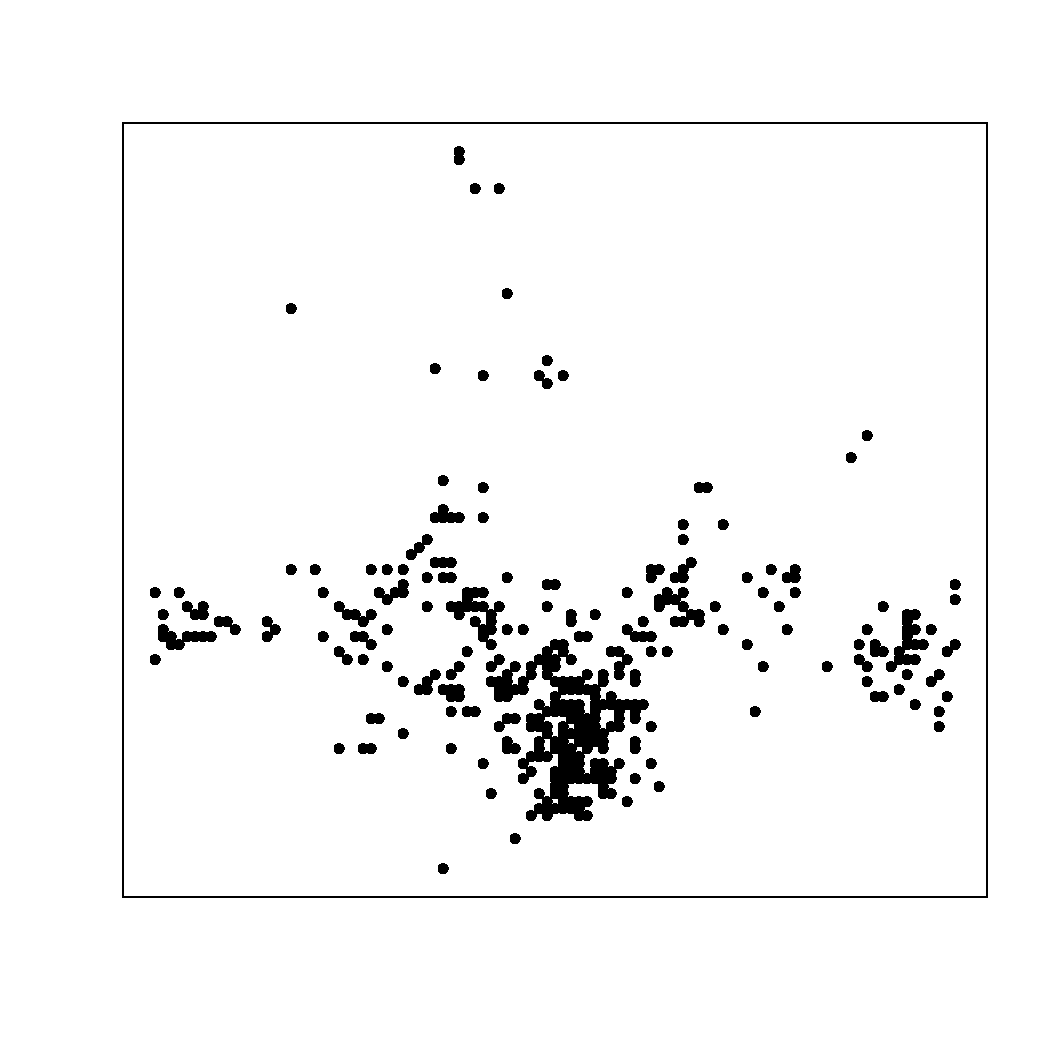
\includegraphics[width=1.9in]{../Figures/example_6C.pdf}
  \caption{}
\end{subfigure}
\caption{Examples of how the habitat patches can be distributed in the different classes of heterogeneous landscapes: a) 0--23\%, b) 24--43\%  and c) 44--100\% located in the middle third of the landscape.}
\label{fig:fig}

\end{figure}

\clearpage

 
%\section*{References}
% The bibtex filename
\bibliographystyle{ecology_letters2}
\bibliography{../../../bibtexFiles/RangeShiftMS.bib}
 
 \end{document}